% =====================================================================
% architecture-figure-v3.tex
% Conference architecture of the micro-encoder router (methods-v3).
% Replaces methods-v2/architecture-figure.tex, which is left unchanged.
%
% Fixes relative to v2 (00-review-findings.md RF-J1..RF-J4):
%   * no \blacktriangledown, \Letter, \dashrightarrow or other glyphs that
%     need amssymb/marvosym; no signal shapes, no Open Triangle tips;
%   * only standard TikZ libraries (positioning, arrows.meta, fit,
%     backgrounds, calc); every style used is defined below;
%   * utility is MODEL-level, U_theta(M|q) (01-model-vs-action-utility.md),
%     mapped to actions through M(a); split depth enters through cost and,
%     only if E0 fails, through the correction Delta (02);
%   * semantic prediction (blue), runtime measurement (orange), training-only
%     teacher (dashed grey) and execution actions (black) are separated;
%   * no continual-learning element (15-conference-vs-journal.md, sec. 7);
%   * no backbone or model names (07: backbone is an engineering decision);
%   * no numbers: nothing in the figure is a measured result.
%
% Notation matches proposed-solution-blue-v3.tex: Eq. (eq:ftheta),
% (eq:kdloss), (eq:route), (eq:feasible), (eq:factor), Alg. 1 and Alg. 2.
%
% Compile standalone:   pdflatex architecture-figure-v3.tex
% Compile record (2026-10-04, see latex-compile.log): compiled with Tectonic
% 0.15.0 (XeTeX engine; no system TeX installed) -> architecture-figure-v3.pdf,
% 0 errors, 0 overfull boxes. pdflatex itself was not available and is not
% claimed.
% Sized for a two-column paper as a full-width figure* (about 17 cm wide):
%   \begin{figure*}[t]\centering
%     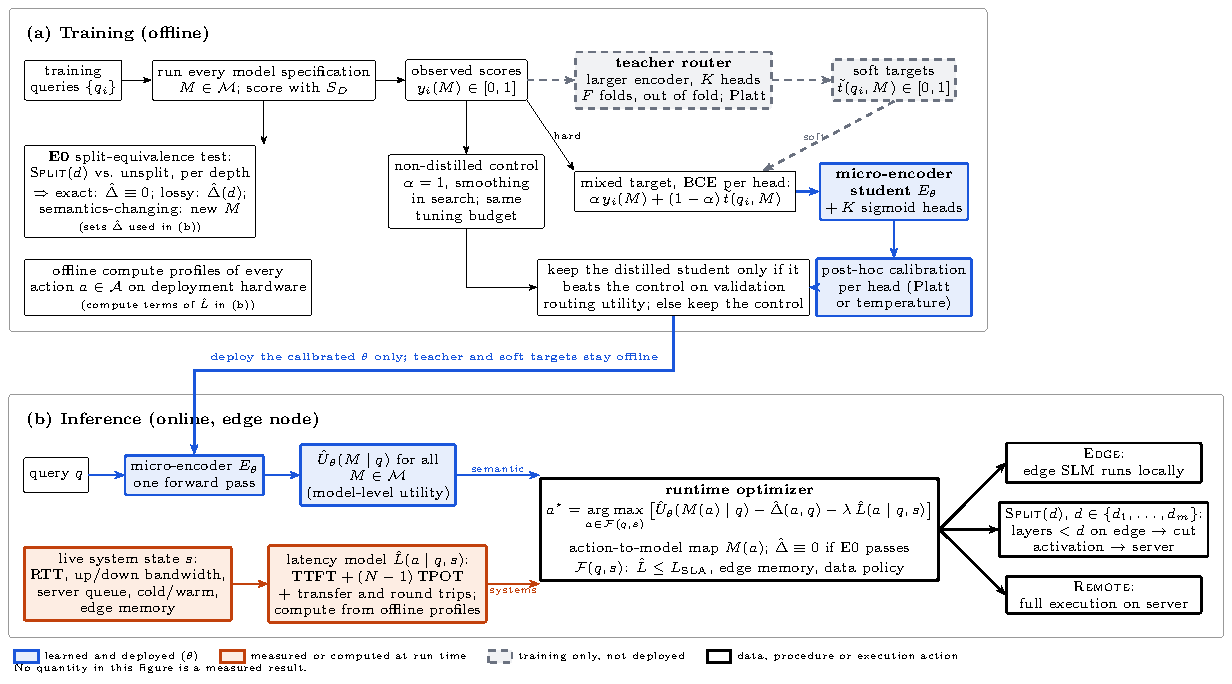
\includegraphics[width=\textwidth]{architecture-figure-v3.pdf}
%     \caption{...}\label{fig:arch}
%   \end{figure*}
% Suggested caption (no citations needed; describes our design only):
%   "Proposed router. (a) Offline: every model specification is run and
%    scored; a larger teacher router, trained out of fold and calibrated,
%    provides soft targets; the micro-encoder student is trained on a mix of
%    observed scores and soft targets and is kept only if it beats a tuned
%    non-distilled control. (b) Online: one encoder pass gives model-level
%    utilities; a latency model fed by live system state gives action costs;
%    the runtime optimizer selects Edge, Split(d) or Remote among feasible
%    actions. The teacher is not deployed."
% =====================================================================
\documentclass[tikz,border=4pt]{standalone}
\usepackage{amsmath}
\usepackage{xcolor}
\usetikzlibrary{positioning,arrows.meta,fit,backgrounds,calc}

\definecolor{learned}{HTML}{1A56DB}    % predicted by the deployed router
\definecolor{learnedfill}{HTML}{E7EEFC}
\definecolor{measured}{HTML}{C2410C}   % measured / computed at run time
\definecolor{measuredfill}{HTML}{FDEDE3}
\definecolor{trainonly}{HTML}{6B7280}  % training only, not deployed
\definecolor{trainfill}{HTML}{F1F2F4}

\begin{document}
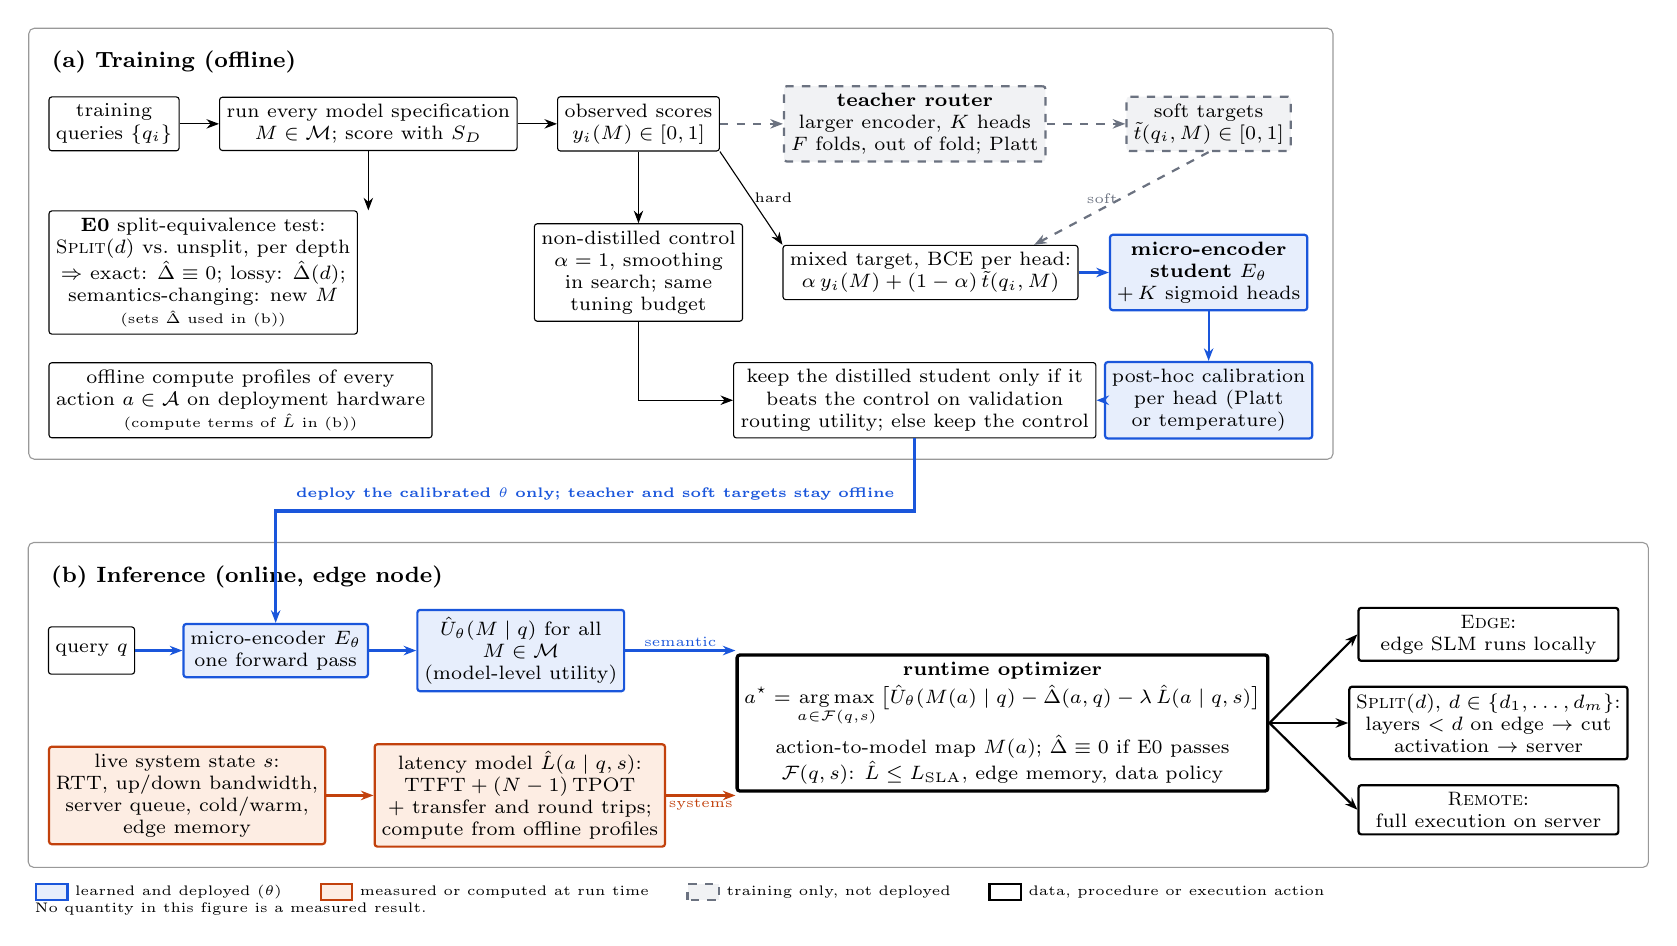
\begin{tikzpicture}[
  font=\scriptsize,
  >={Stealth[length=1.6mm]},
  box/.style      ={draw=black, thin, rounded corners=1pt, fill=white,
                    align=center, inner sep=2.5pt, minimum height=6mm},
  learnedbox/.style ={box, draw=learned, thick, fill=learnedfill},
  measuredbox/.style={box, draw=measured, thick, fill=measuredfill},
  trainbox/.style ={box, draw=trainonly, thick, dashed, fill=trainfill},
  actionbox/.style={box, thick, fill=white},
  optbox/.style   ={box, very thick, fill=white},
  flow/.style     ={->, thin},
  flowL/.style    ={->, thick, learned},
  flowM/.style    ={->, thick, measured},
  flowT/.style    ={->, thick, dashed, trainonly},
  deploy/.style   ={->, very thick, learned},
  paneltitle/.style={font=\footnotesize\bfseries, anchor=west, inner sep=1pt},
  note/.style     ={font=\tiny, align=center, inner sep=1pt},
]

% =====================================================================
% (a) TRAINING (offline)
% =====================================================================
% row 1: run and score -> observed scores -> teacher -> soft targets
\node[box, anchor=west] (q) at (0,0)
  {training\\queries $\{q_i\}$};
\node[box, right=5mm of q] (run)
  {run every model specification\\$M\in\mathcal{M}$; score with $S_D$};
\node[box, right=5mm of run] (y)
  {observed scores\\$y_i(M)\in[0,1]$};
\node[trainbox, right=8mm of y] (teacher)
  {\textbf{teacher router}\\larger encoder, $K$ heads\\$F$ folds, out of fold; Platt};
\node[trainbox, right=10mm of teacher] (soft)
  {soft targets\\$\tilde t(q_i,M)\in[0,1]$};
\node[paneltitle, anchor=south west] (Ta) at ($(q.north west)+(0,0.25)$)
  {(a) Training (offline)};

% row 2: E0, non-distilled control, mixed target, student
\node[box, anchor=north west] (e0) at ($(q.south west)+(0,-0.75)$)
  {\textbf{E0} split-equivalence test:\\$\textsc{Split}(d)$ vs.\ unsplit, per depth\\
   $\Rightarrow$ exact: $\hat\Delta\equiv 0$; lossy: $\hat\Delta(d)$;\\
   semantics-changing: new $M$\\{\tiny (sets $\hat\Delta$ used in (b))}};
\node[box] (ctrl) at ($(y |- e0)+(0,0)$)
  {non-distilled control\\$\alpha=1$, smoothing\\in search; same\\tuning budget};
\node[box] (loss) at ($(teacher |- e0)+(0.2,0)$)
  {mixed target, BCE per head:\\$\alpha\,y_i(M)+(1-\alpha)\,\tilde t(q_i,M)$};
\node[learnedbox] (student) at (soft |- e0)
  {\textbf{micro-encoder}\\\textbf{student} $E_\theta$\\$+\,K$ sigmoid heads};

% row 3: profiles, selection gate, calibration
\node[box, anchor=north west] (prof) at ($(e0.south west)+(0,-0.35)$)
  {offline compute profiles of every\\action $a\in\mathcal{A}$ on deployment hardware\\{\tiny (compute terms of $\hat L$ in (b))}};
\node[box] (gate) at (teacher |- prof)
  {keep the distilled student only if it\\beats the control on validation\\routing utility; else keep the control};
\node[learnedbox] (calib) at (soft |- prof)
  {post-hoc calibration\\per head (Platt\\or temperature)};

% training edges
\draw[flow]  (q) -- (run);
\draw[flow]  (run) -- (y);
\draw[flowT] (y) -- (teacher);
\draw[flowT] (teacher) -- (soft);
\draw[flow]  (run.south) -- (run.south |- e0.north);
\draw[flow]  (y.south) -- (ctrl.north);
\draw[flow]  (y.south east) -- node[note, right]{hard} (loss.north west);
\draw[flowT] (soft.south) -- node[note, left, text=trainonly]{soft} ($(loss.north east)!0.3!(loss.north)$);
\draw[flowL] (loss) -- (student);
\draw[flowL] (student) -- (calib);
\draw[flowL] (calib) -- (gate);
\draw[flow]  (ctrl.south) |- (gate.west);

\begin{pgfonlayer}{background}
  \node[draw=black!40, rounded corners=2pt, inner sep=2.5mm,
        fit=(Ta)(q)(run)(y)(teacher)(soft)(e0)(ctrl)(loss)(student)(prof)(gate)(calib)]
        (panelA) {};
\end{pgfonlayer}

% =====================================================================
% (b) INFERENCE (online, edge node)
% =====================================================================
\coordinate (bTop) at ($(panelA.south west)+(0.25,-1.3)$);
\node[paneltitle, anchor=north west] (Tb) at (bTop)
  {(b) Inference (online, edge node)};

% semantic path
\node[box, anchor=north west] (qq) at ($(Tb.south west)+(0,-0.45)$)
  {query $q$};
\node[learnedbox, right=6mm of qq] (enc)
  {micro-encoder $E_\theta$\\one forward pass};
\node[learnedbox, right=6mm of enc] (U)
  {$\hat U_\theta(M\mid q)$ for all\\$M\in\mathcal{M}$\\(model-level utility)};

% systems path
\node[measuredbox, anchor=north west] (state) at ($(qq.south west)+(0,-0.9)$)
  {live system state $s$:\\RTT, up/down bandwidth,\\server queue, cold/warm,\\edge memory};
\node[measuredbox, right=6mm of state] (lat)
  {latency model $\hat L(a\mid q,s)$:\\$\mathrm{TTFT}+(N-1)\,\mathrm{TPOT}$\\$+$ transfer and round trips;\\compute from offline profiles};

% runtime optimizer, vertically between the two paths
\coordinate (mid) at ($(U.center)!0.5!(lat.center)$);
\coordinate (optW) at ($(U.east |- mid)+(1.4,0)$);
\node[optbox, anchor=west] (opt) at (optW)
  {\textbf{runtime optimizer}\\[2pt]
   $\displaystyle a^\star=\operatorname*{arg\,max}_{a\in\mathcal{F}(q,s)}
   \big[\hat U_\theta(M(a)\mid q)-\hat\Delta(a,q)-\lambda\,\hat L(a\mid q,s)\big]$\\[2pt]
   action-to-model map $M(a)$; $\hat\Delta\equiv 0$ if E0 passes\\
   $\mathcal{F}(q,s)$: $\hat L\le L_{\mathrm{SLA}}$, edge memory, data policy};

% execution actions
\node[actionbox, minimum width=33mm, right=10mm of opt] (split)
  {$\textsc{Split}(d)$, $d\in\{d_1,\dots,d_m\}$:\\layers $<d$ on edge $\to$ cut\\activation $\to$ server};
\node[actionbox, minimum width=33mm, above=3mm of split] (edge)
  {$\textsc{Edge}$:\\edge SLM runs locally};
\node[actionbox, minimum width=33mm, below=3mm of split] (remote)
  {$\textsc{Remote}$:\\full execution on server};

% inference edges
\draw[flowL] (qq) -- (enc);
\draw[flowL] (enc) -- (U);
\draw[flowM] (state) -- (lat);
\draw[flowL] (U.east) -- node[note, above, sloped, text=learned]{semantic} (opt.west |- U.east);
\draw[flowM] (lat.east) -- node[note, below, sloped, text=measured]{systems} (opt.west |- lat.east);
\draw[flow, thick] (opt.east) -- (edge.west);
\draw[flow, thick] (opt.east) -- (split.west);
\draw[flow, thick] (opt.east) -- (remote.west);

\begin{pgfonlayer}{background}
  \node[draw=black!40, rounded corners=2pt, inner sep=2.5mm,
        fit=(Tb)(qq)(enc)(U)(state)(lat)(opt)(edge)(split)(remote)]
        (panelB) {};
\end{pgfonlayer}

% deployment: only the selected, calibrated student crosses to panel (b)
\draw[deploy] (gate.south) -- ($(gate.south |- panelA.south)+(0,-0.65)$)
  -| (enc.north)
  node[pos=0.25, above, font=\tiny\bfseries, text=learned]
  {deploy the calibrated $\theta$ only; teacher and soft targets stay offline};

% =====================================================================
% Legend
% =====================================================================
\node[anchor=north west, font=\tiny, inner sep=1pt, align=left]
  (leg) at ($(panelB.south west)+(0.05,-0.15)$) {%
  \tikz[baseline=-0.6ex]{\draw[learned, thick, fill=learnedfill] (0,-0.1) rectangle (0.4,0.1);}~learned and deployed ($\theta$)\qquad
  \tikz[baseline=-0.6ex]{\draw[measured, thick, fill=measuredfill] (0,-0.1) rectangle (0.4,0.1);}~measured or computed at run time\qquad
  \tikz[baseline=-0.6ex]{\draw[trainonly, thick, dashed, fill=trainfill] (0,-0.1) rectangle (0.4,0.1);}~training only, not deployed\qquad
  \tikz[baseline=-0.6ex]{\draw[black, thick, fill=white] (0,-0.1) rectangle (0.4,0.1);}~data, procedure or execution action\\
  No quantity in this figure is a measured result.};

\end{tikzpicture}
\end{document}
